\section{Terrain and Navigation}

In order to give the user the freedom to model any type of virtual world, providing the ability to specify any type of base terrain is essential. Efficiently rendering and navigating this terrain is also key for both the user experience and visual realism. How our system manages these requirements are discussed sections \textit{Loading Terrain}, \textit{Rendering Terrain} and \textit{Navigating Terrain} below.

\subsection{Loading Terrain}

As stated previously, our work focuses on terrain content and not terrain relief modelling. As such, the user is only able to load a static, pre-generated terrain in the form of a Terragen height-map. A height-map is a 2-dimensional grid of height values which, once loaded and converted, represents the height of the terrain on a regular grid. The Terragen file format is a freely available and widely used file-specification created by PlanetSide \protect\footnotemark \footnotetext{\url{http://www.planetside.co.uk}} for their realistic virtual world generation software, Terragen. The format wraps raw height data with other important information essential to accurate rendering such as base height, scales and dimensions.\\
Note that modelling the base terrain as static is a simplification as in reality it is affected by erosion. The extent of which depends on many factors including wind, vegetation and water.

\subsection{Rendering Terrain}

Once parsed, the height-map data is transferred to the GPU as a two dimensional texture for rendering. In order to better visualize the terrain relief, a Blinn–Phong shading model is used when rendering the terrain.
This shading model takes into consideration camera viewpoint and lighting incidence angles to determine the influence of diffuse and specular lighting on individual terrain vertices. This information is subsequently used to calculate a weighted contribution of ambient, specular and diffuse colors to determine the aggregate color of individual terrain vertices. By accurately modelling specular and diffuse highlights, renders are more realistic and shapes more distinguishable \citep{Blinn}. By employing this model in this work, terrain relief is made clear.\\
Essential to the Blinn-Phong shading model are the normal vectors for each terrain vertex. This is done using the algorithm outlined in equation \ref{eq:normals_calculation} and illustrated in figure \ref{fig:normals_calculation}. Each normal is calculated in parallel on the GPU, thus ensuring real-time results.

\begin{equation} \label{eq:normals_calculation}
N_{P} = V_{ac} \times V_{db}
\end{equation}
Where: $N_{P}$ is the normal vector at point P and $P_{A}$, $P_{B}$, $P_{C}$ and $P_{D}$ are the direct points surrounding P in the X and Y direction (see figure \ref{fig:normals_calculation}).

\begin{figure}[h]
\center
	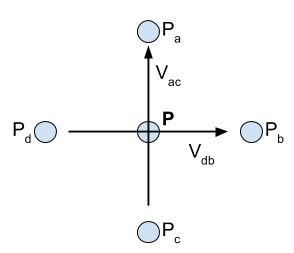
\includegraphics[width=\textwidth/2]{normals_calculation.png}
	\caption{\textit{Illustration of the vertices and vectors used to calculate terrain normal at position \textit{P}.}}
	\label{fig:normals_calculation}
\end{figure}

\subsection{Navigation}

In order for users to successfully and intuitively navigate through virtual worlds, it is important to prevent disorientation by ensuring continuous user awareness of location and orientation \cite{Darken1993}. 
In their work, Darken et al. \cite{Darken1993} explore various navigation techniques to do so, including the flying scenario where users explore virtual worlds as if they were flying through it. This navigation technique provides a birds eye view of the virtual worlds and enables users to gain an overview of the terrain and efficiently locate landmarks to serve as point of references. Locating such landmarks proves extremely useful in keeping the user aware of his location and therefore preventing disorientation \cite{Darken1993}. Birds eye has become the most widespread navigation technique employed in video games, simulators and virtual world generation software. In order to support a variety of users (novice to computer graphic experts), this is the navigation style used in our system. To further prevent disorientation, a compass is continuously displayed stating the current heading. \\

Intuitive controls and suitable sensitivity thereof are also essential. The correlation between key-press and mouse movement must be predictable so that the user can navigate in three dimensional space without losing his bearings. In an attempt to cater for the control requirements of a wider user-base, two different control types are available in this system: \textit{keyboard-driven} and \textit{click-and-drag}. Details of which can be found in table \ref{tab:control_types}. The active control type is easily configurable, along with sensitivity parameters, through the application's configuration interface.

\begin{table}[h]	
  \centering
	    \begin{tabular}{|p{2.5cm}|p{2.25cm}|p{2.25cm}|p{2.25cm}|p{2.25cm}|p{2.25cm}|}
  	    \hline	
  	    \textbf{Control-type} & \textbf{Translate Left/Right} & \textbf{Translate Up/Down} & \textbf{Translate Front/Back} & \textbf{Rotate Left/Right} & \textbf{Rotate Up/Down} \\
		\hline
		\textbf{First-Person} & A/D key-press & - & W/S key-press & Horizontal mouse movement & Vertical mouse movement \\
		\hline
		\textbf{Click-and-drag} & Horizontal click \& drag & Vertical click \& drag & Scroll wheel & Ctrl + horizontal click \& drag & Ctrl + vertical click \& drag\\
		\hline
		\end{tabular}
		\caption{Control types instruction sheet}
		\label{tab:control_types}
\end{table}

